\documentclass[10pt,letterpaper]{article}
\usepackage[margin=0.7in]{geometry}
\usepackage[T1]{fontenc}
\usepackage{lmodern}
\usepackage{microtype}
\usepackage{graphicx}
\usepackage{booktabs,array,tabularx}
\usepackage{caption}
\usepackage{titlesec}
\usepackage{xurl}
\usepackage[hidelinks,pdftitle={Smaller RAM for the Same Model},pdfauthor={Sadad Haidari and Rommel Mendez-Lopez}]{hyperref}
\pagestyle{empty}
\setlength{\parindent}{1em}
\setlength{\parskip}{3pt}
\setlength{\emergencystretch}{1.5em}
\titleformat{\section}{\normalfont\large\bfseries}{\thesection}{0.6em}{}
\titlespacing*{\section}{0pt}{10pt plus 1pt minus 1pt}{4pt}
\captionsetup{font=small,labelfont=bf,labelsep=period,skip=5pt}
\urlstyle{same}
\newcolumntype{L}[1]{>{\raggedright\arraybackslash}p{#1}}
\begin{document}
\begin{center}
{\LARGE Smaller RAM for the Same Model\par}
\vspace{6pt}
{\large Sadad Haidari \quad and\quad Rommel Mendez-Lopez\par}
\vspace{4pt}
Computer Architecture, Project Review\\
27 Oct 2026
\end{center}
\vspace{-5pt}
\section{Goal and result}
The goal is to run frontier-class models on less hardware. Model weights are the stored numbers that guide a model's responses. Those weights can exceed a device's RAM before its CPU starts useful work. We test lossless compression in the processor-to-RAM path: pack the weights in RAM, then restore their original BF16 bits before CPU math.

On a complete converted 2B text model, packing cuts peak process RAM from 3.99 GB to 3.06 GB. Generation rises from 15.95 to 19.92 tokens/s at 12 CPU threads. A token is a short text unit. Under a 4.5 GB process allocation cap, the raw model fails to load and the packed model runs. These are CPU measurements. The FPGA has separate simulation and logic-mapping results.

The original proposal fetched extra weight bits when an error bound required them. It retained the full weight store. This report tests compressed storage instead; the adaptive fetch controller is not evaluated.

\section{Processor-to-RAM path}
The FPGA tests a compression unit between a processor and RAM. On a write, an encoder packs a block. On a read, a decoder restores that block before the processor computes. The processor still sees the original weights. The FPGA does not need to hold or run the whole model. Figure 1 separates the live CPU test from the circuit test.

\par\noindent\begin{minipage}{\linewidth}
\centering
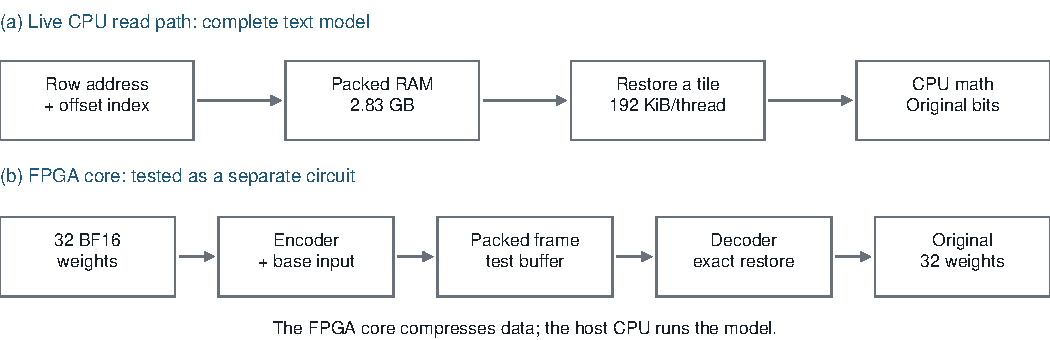
\includegraphics[width=\linewidth]{figure-1.pdf}
\captionof{figure}{The CPU test keeps packed weights in RAM and restores small tiles on demand. Its 192 KiB per thread consists of a 64 KiB scratch buffer and a 128 KiB row cache. The FPGA bench checks the encoder, a test frame buffer and the decoder. A host selects each tensor's base; a board RAM interface remains to be built.}
\end{minipage}
\par\vspace{3pt}
\section{Block format}
BF16 stores each weight in 16 bits: one sign bit, eight exponent bits and seven fraction bits. The exponent sets the scale of the number. Most exponents in each tested weight matrix lie in a small range. We replace those eight bits with a four-bit offset in that range. An escape code stores the full exponent when it does not fit. Sign and fraction bits remain intact.

For 32 weights, the common block shrinks from 64 B to 48 B, plus one extra 8-bit field per escape. A row index permits direct access. A row remains raw if packing would enlarge it. Including the row index, the weight store shrinks from 3.765 GB to 2.829 GB, a 24.84\% reduction. Adding 18,489 B for archive headers gives the full file size. This preserves BF16 weights. The installed eight-bit model is smaller still; this test does not improve its compression.

\newpage
\section{CPU results}
Both modes load the same 320 tensors from the same converted BF16 text model [3]. The baseline comes from the publisher BF16 checkpoint. Both modes omit the same vision and extra prediction components. The storage comparison excludes those components from both modes.

\par\noindent\begin{minipage}{\linewidth}
\centering
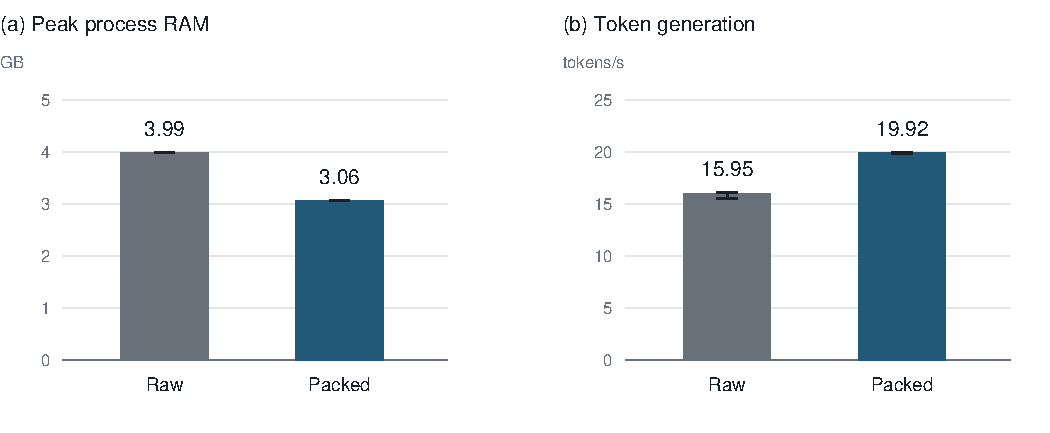
\includegraphics[width=\linewidth]{figure-2.pdf}
\captionof{figure}{Medians of three fresh-process pairs; thin lines span the three observations. Axes start at zero. RAM is the Windows peak working set through inference, before score-file export. Generation rate excludes model load, prompt processing and score export. GB = 10\textsuperscript{9} B.}
\end{minipage}
\par\vspace{3pt}
\par\vspace{3pt}
{\small\noindent\begin{tabular}{@{}L{0.410714\dimexpr\linewidth-12pt\relax}L{0.589286\dimexpr\linewidth-12pt\relax}@{}}
\toprule
\textbf{Measured check} & \textbf{Result} \\
\midrule
Native full-store restore & 320 unique tensors; all 3,764,747,520 B match \\
Model output checks & 49,167,360 exact score comparisons across repeats; 12,167,680 more on a longer input \\
\bottomrule
\end{tabular}\par}
\vspace{3pt}
The score check compares the stored bits of each output float. The three repeats use the same two 32-token sequences, so the 49.2 million count includes repeated scores. A separate input has 327 prompt tokens and 48 generated tokens. All scores match the raw mode in the same native build. Each run uses the complete converted text model.

\section{Allocation limit}
We limited each process to 4.5 GB of private committed allocations [5]. Raw mode failed to allocate its 3.765 GB weight buffer. Packed mode completed inference, with a 4.024 GB peak committed allocation. The cap includes more than resident RAM, so this is an allocation-budget test on this PC. It is not a test on a different device.

\section{Test setup}
Host: AMD Ryzen 9 7900X, 32 GB RAM. GPU work: none. Both modes use the same CPU build of llama.cpp [4], 512 context slots, batches of 32 and 12 threads. We disable mapped weights and extra buffer kernels. The RAM count includes the runner, model state, decoder buffers and retained test scores. Model-load cost and prompt time are recorded in the evidence; the plotted speed measures token generation.

\newpage
\section{Circuit tests}
The RTL encoder and decoder pass 68,056 frames: all 65,536 possible BF16 bit patterns, 1,024 random blocks and 1,496 blocks drawn from 187 real weight matrices. The bench checks exact bits, held outputs under stalls, reset aborts, invalid frame lengths, invalid bases and 16 consecutive accepted frames. A separate native test places all BF16 bit patterns in compressed rows.

Yosys maps the paired circuits to 7,537 LUT cells and 1,170 flip-flops, with no DSP or block RAM. This is a logic estimate for the 7-series target. It excludes a board interface and frame storage. The wide frame bus is internal. The circuit is not placed or routed, and no clock rate, power or board bandwidth has been measured.

The target is the Zybo Z7-20 [6]. The current full archive comes from the software reference. The FPGA has not produced that archive or supplied data to the running CPU. The board still needs a RAM interface and host connection.

\section{Decode cost and next tests}
\par\vspace{3pt}
{\small\noindent\begin{tabular}{@{}L{0.158730\dimexpr\linewidth-36pt\relax}L{0.198413\dimexpr\linewidth-36pt\relax}L{0.214286\dimexpr\linewidth-36pt\relax}L{0.428571\dimexpr\linewidth-36pt\relax}@{}}
\toprule
\textbf{CPU threads} & \textbf{Raw tokens/s} & \textbf{Packed tokens/s} & \textbf{What the test shows} \\
\midrule
2 & 14.69 & 6.13 & CPU decode cost dominates. \\
6 & 15.65 & 15.91 & Rates are close in this short probe. \\
12 & 15.95 & 19.92 & Faster in three paired runs. \\
\bottomrule
\end{tabular}\par}
\vspace{3pt}
At two threads, packing cuts RAM but slows generation. Dedicated decode logic could remove that CPU work. Next, stream blocks through a narrow bus, place a FIFO on each side and overlap reads with decoding. A FIFO holds completed blocks while the next unit stalls. Measure stalled clocks at each interface to check whether the circuit improves the read rate.

The 12-thread gain is consistent with less data movement, but we did not measure DRAM transactions or CPU stall counters. Cache effects and decode cost also change the rate. To test the cause, record requested and returned data (B), clocks with no data in the FIFO, and clocks spent in the decoder. These counters distinguish slow RAM from slow restoration.

\section{Compression limits}
This format can approach a 25\% weight reduction when most exponents fit the chosen range. It cannot deliver a tenfold reduction. If a 100 GB BF16 weight store had the same statistics, it would need about 75 GB after packing, before model state and other buffers. That is a conditional estimate, not a frontier-model result. Eight-bit model weights can be smaller still, but change the precision target.

Lossless weight compression and hardware decoders exist in prior work [1,2]. We implemented the block format and RTL, added a row decoder to llama.cpp, and tested restored tensor bits and model outputs. The inference engine and tensor math come from llama.cpp [4]. A board-connected block store with measured timing remains to be tested.

\newpage
\section*{References and evidence}
{\small\noindent [1] P. Yubeaton et al. \textit{Huff-LLM: End-to-End Lossless Compression for Efficient LLM Inference}.\newline \url{https://arxiv.org/abs/2502.00922}\newline Prior work on hardware decoders for lossless weight compression.\par}
\vspace{4pt}
{\small\noindent [2] R. Fan et al. \textit{ZipServ: Fast and Memory-Efficient LLM Inference with Hardware-Aware Lossless Compression}.\newline \url{https://arxiv.org/abs/2603.17435}\newline Prior work on fast inference from compressed model weights.\par}
\vspace{4pt}
{\small\noindent [3] Qwen. \textit{Qwen3.5-2B}.\newline \url{https://huggingface.co/Qwen/Qwen3.5-2B}\newline Publisher BF16 weights. Vision and MTP excluded from both modes.\par}
\vspace{4pt}
{\small\noindent [4] ggml-org. \textit{llama.cpp}.\newline \url{https://github.com/ggml-org/llama.cpp}\newline Inference engine and tensor math. Both modes use the same CPU build with the project row decoder.\par}
\vspace{4pt}
{\small\noindent [5] Microsoft. \textit{JOBOBJECT\_EXTENDED\_LIMIT\_INFORMATION}.\newline \url{https://learn.microsoft.com/en-us/windows/win32/api/winnt/ns-winnt-jobobject_extended_limit_information}\newline Defines the private committed-allocation limit used for the 4.5 GB fit test.\par}
\vspace{4pt}
{\small\noindent [6] Digilent. \textit{Zybo Z7 Board Reference Manual}.\newline \url{https://digilent.com/reference/_media/reference/programmable-logic/zybo-z7/zybo-z7_rm.pdf}\newline Target board documentation. No board run or routed timing in this report.\par}
\vspace{4pt}
\section*{Project code}
\noindent\url{https://github.com/sadadhaidari/computer-architecture-bf16-compression}\par
The repo contains the block codec, RTL encoder and decoder, and a small testbench. The tests run without downloading a model. The CPU measurements in this report come from the full-model experiment; the repo does not include its complete inference build.

\end{document}
